% Embed2Heights --- final solution, detailed walkthrough
% Compile:  tectonic framework_overview.tex   (needs architecture.pdf alongside)
\documentclass[aspectratio=169,11pt]{beamer}

\usetheme{metropolis}
\usepackage[T1]{fontenc}
\usepackage{booktabs}
\usepackage{amsmath}
\usepackage{xcolor}
\usepackage{tikz}
\usetikzlibrary{positioning,arrows.meta,fit,calc,backgrounds}

\definecolor{cAlpha}{HTML}{1b6ca8}
\definecolor{cToken}{HTML}{c8553d}
\definecolor{cHead} {HTML}{2a7f62}
\definecolor{cOut}  {HTML}{6a4c93}
\definecolor{cGray} {HTML}{555555}

% ---- compact in-slide schematic styles ----
\tikzset{
  >={Stealth[length=2mm]},
  sbox/.style={rounded corners=1.5pt,draw,align=center,inner sep=2.5pt,
               font=\scriptsize,minimum height=0.6cm},
  spix/.style={sbox,fill=cAlpha!12,draw=cAlpha},
  stok/.style={sbox,fill=cToken!12,draw=cToken},
  shd/.style ={sbox,fill=cHead!12,draw=cHead},
  sop/.style ={sbox,fill=cOut!14,draw=cOut},
  sar/.style ={->,semithick,cGray},
}

\newcommand{\fit}{\textcolor{cHead}{\textbf{Fits:}}\ }
\newcommand{\code}[1]{\texttt{\small #1}}

\title{Reaching new heights with GeoFM}
% \subtitle{Gating four frozen GFMs, then restoring the object edges their embeddings blur away}
\author{Team: Attention\_Plzzz\\[2pt]
  \small Dingqi Ye, Daniel Kiv, Wen Zhou, Wei Hu, Ayush Khot}
\institute{CyberGIS Center for Advanced Digital and Spatial Studies\\
  University of Illinois at Urbana-Champaign}
\date{\today}

\begin{document}

\maketitle

\begin{frame}{Roadmap}\tableofcontents\end{frame}

% =====================================================================
\section{Task \& Inputs}
% =====================================================================

\begin{frame}{The task}
  Per $256\times256$ tile, predict 4 channels:
  \[\big[\text{building},\ \text{vegetation},\ \text{water},\ \text{height (m)}\big]\]
  ch\,0--2 = binary presence \quad ch\,3 = continuous height.

  \vspace{0.5em}
  \begin{center}\small
  \begin{tabular}{lccccc}
    \toprule
    & IoU bld & IoU tree & IoU water & RMSE bld$_H$ & RMSE veg$_H$\\
    \midrule
    weight & 25\% & 15\% & 15\% & 25\% & 20\%\\
    \bottomrule
  \end{tabular}
  \end{center}
  \footnotesize Score $=\sum_i w_i\,\text{IoU}_i+\sum_j w_j\max(0,1-\text{RMSE}_j/X_j)$,
  $X_{\text{bld}}{=}3$m, $X_{\text{veg}}{=}5$m.

  \vspace{0.5em}
  \normalsize\alert{Everyone gets the \emph{same} frozen embeddings.}
  No raw imagery $\Rightarrow$ a score gap is a \textbf{method} gap.
\end{frame}

\begin{frame}{The inputs: two families of embedding}
  \begin{center}\small
  \begin{tabular}{llcl}
    \toprule
    Embedding & Source & Shape & Note\\
    \midrule
    \textcolor{cAlpha}{AlphaEarth} & multi-sensor & $64\times256^2$ & dense, full-res\\
    \textcolor{cAlpha}{Tessera}    & multi-sensor & $128\times256^2$ & dense, full-res\\
    \textcolor{cToken}{TerraMind S1/S2} & SAR / optical & $768\times16^2$ & post-encoder tokens\\
    \textcolor{cToken}{Thor S1/S2}      & SAR / optical & $768\times16^2$ & raw scale $\pm17$k\\
    \bottomrule
  \end{tabular}
  \end{center}

  \vspace{0.6em}
  \begin{columns}[T]
    \begin{column}{0.5\textwidth}
      \textcolor{cAlpha}{\textbf{Dense, full-res}}\\
      \footnotesize per-pixel features $\to$ boundaries \& texture (drives IoU).
    \end{column}
    \begin{column}{0.5\textwidth}
      \textcolor{cToken}{\textbf{Coarse tokens ($16^2$)}}\\
      \footnotesize $16\times$ downsampled $\to$ global semantics, no detail.
    \end{column}
  \end{columns}

  \vspace{0.5em}
  \footnotesize This split --- dense vs.\ coarse --- dictates the whole design.
\end{frame}

\begin{frame}{The labels (and how the metric reads them)}
  Target tensor per pixel: $[\,c_{\text{bld}},\,c_{\text{veg}},\,c_{\text{water}},\,h/30\,]$
  \begin{itemize}
    \item ch\,0--2: \textbf{coverage fractions} $c\in[0,1]$ (a 10\,m pixel is rarely pure).
    \item ch\,3: nDSM \textbf{height} in metres, normalised by 30.
    \item \code{valid\_mask}: separate global (nodata) + height (nDSM holes) masks.
  \end{itemize}
  \vspace{0.4em}
  How the metric binarises them --- and why it matters later:
  \begin{itemize}
    \item \textbf{IoU} compares \code{pred>0.5} vs.\ official GT $=\code{coverage}>0.10$.
    \item \textbf{RMSE} is masked \emph{per class} (only pixels of that class count).
  \end{itemize}
\end{frame}

% =====================================================================
\section{Data observations}
% =====================================================================

\begin{frame}{Two label defects we found --- and masked}
  Auditing the GT surfaced two \emph{systematic} defects. Both are handled by the
  two-channel \code{valid\_mask}, so a defect never becomes a wrong training signal.
  \begin{center}\small
  \begin{tabular}{lll}
    \toprule
    Defect & What we see & How we handle it\\
    \midrule
    \textbf{nDSM holes} & height $=0$ on labelled objects & drop px from \emph{height} loss;\\
      & (often whole sub-tiles) & keep presence\\[2pt]
    \textbf{Deleted footprints} & building label empty where & drop px from \emph{presence/seg} loss;\\
      & nDSM\,+\,embeddings say building & keep height\\
    \bottomrule
  \end{tabular}
  \end{center}
  \begin{itemize}\small
    \item \code{valid\_mask} $=$ 2 channels: (0) global/presence, (1) height.
    \item Each defect zeroes \emph{only} its channel $\Rightarrow$ the other task keeps learning.
  \end{itemize}
\end{frame}

\begin{frame}{Observation A: nDSM holes \hfill\small\textcolor{cGray}{height label}}
  \begin{center}
  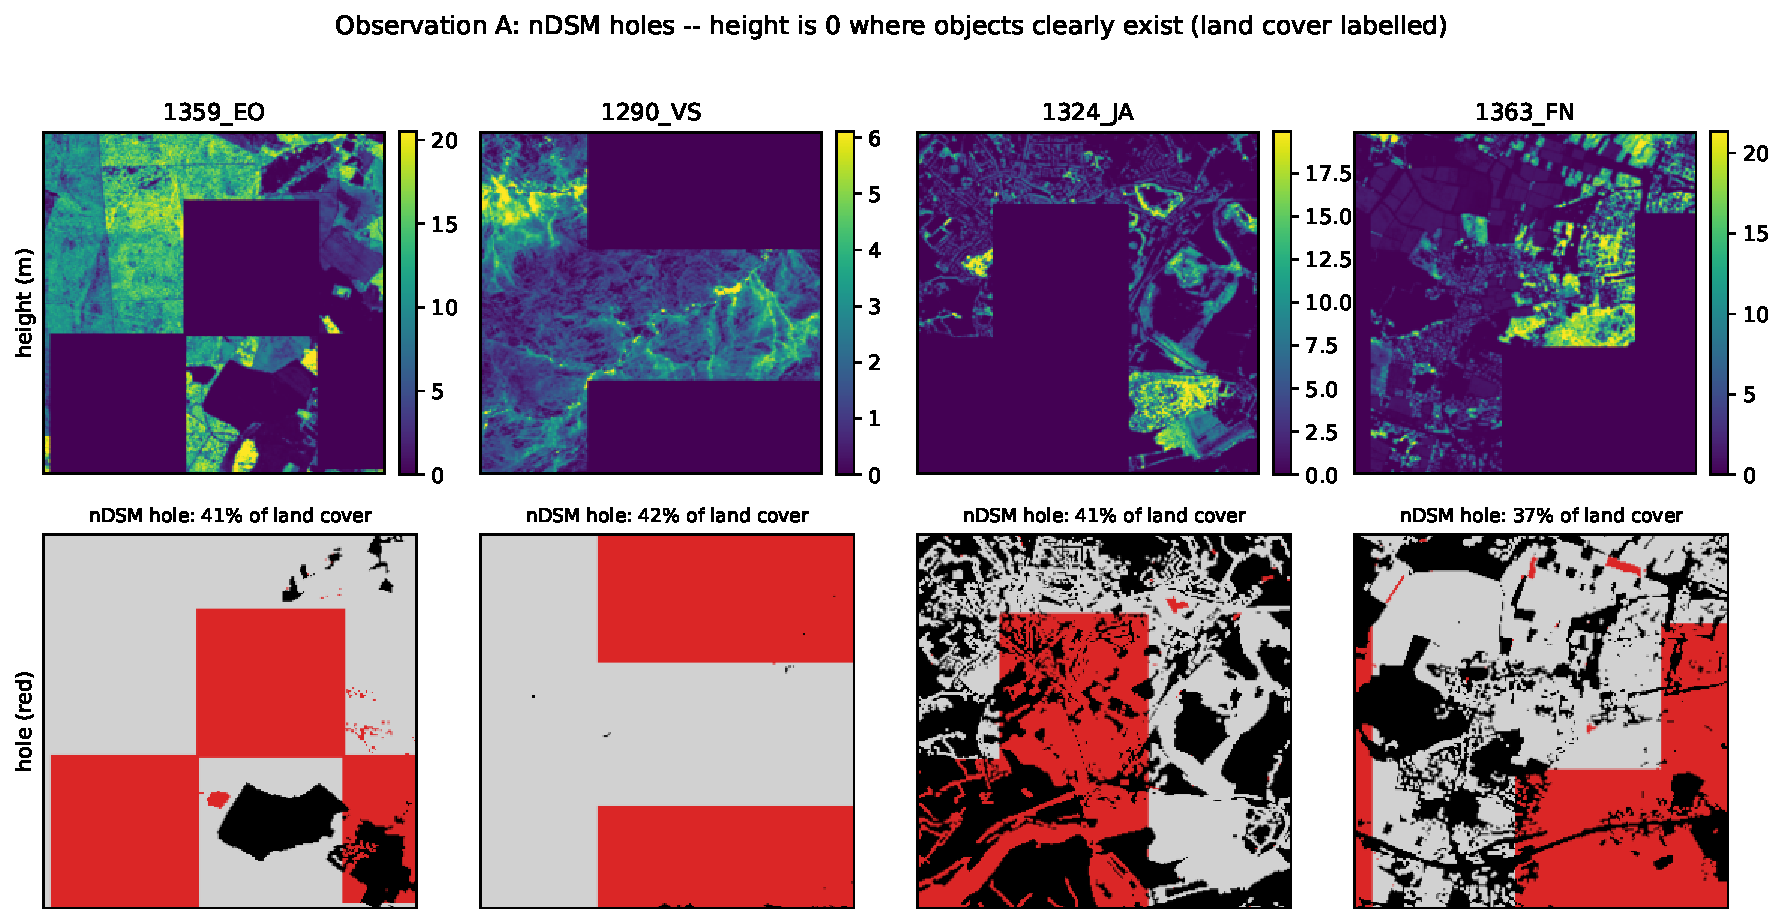
\includegraphics[width=\textwidth,height=0.58\textheight,keepaspectratio]{fig_height_holes.pdf}
  \end{center}
  {\footnotesize Top: nDSM height as stored (the label writes a literal $0$ $\to$ dark).
   Bottom: red $=$ labelled land cover with height $=0$ (up to $\sim$40\% of px).
   \fit \code{ndsm\_hole = height==0 \& has\_landcover} $\to$ dropped from height RMSE
   only; presence kept.}
\end{frame}

\begin{frame}{Observation B: deleted building footprints \hfill\small\textcolor{cGray}{presence label}}
  \begin{center}
  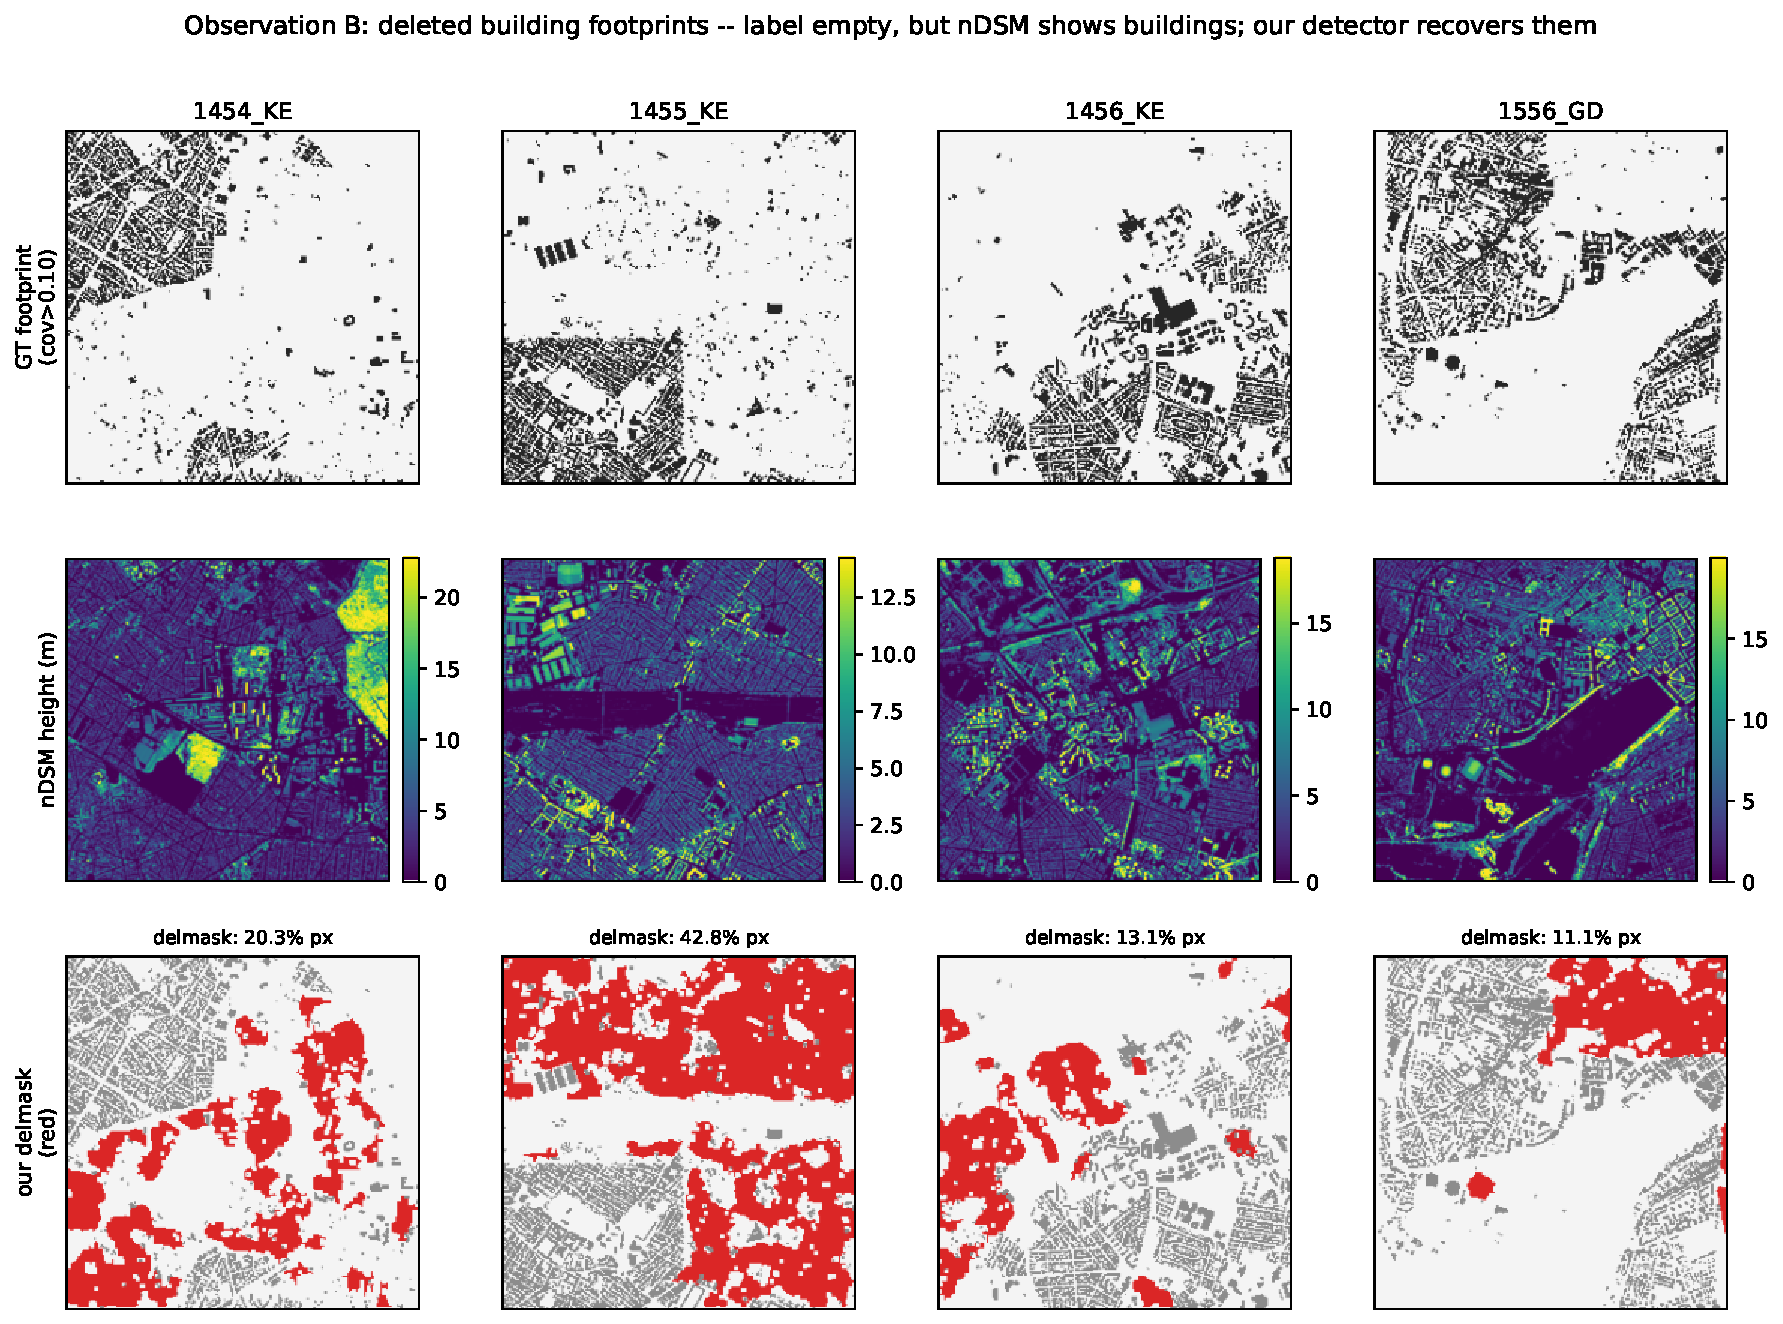
\includegraphics[width=\textwidth,height=0.64\textheight,keepaspectratio]{fig_building_holes.pdf}
  \end{center}
  {\footnotesize Footprint empty (top) where the nDSM (mid) shows buildings; a density-gap
   detector (blob $\ge50$px) recovers the region (red, bottom).
   \fit dropped from presence/seg loss, height kept --- never punish a \emph{correct} building.}
\end{frame}

% =====================================================================
\section{Architecture}
% =====================================================================

\begin{frame}{Architecture at a glance}
  \centering
  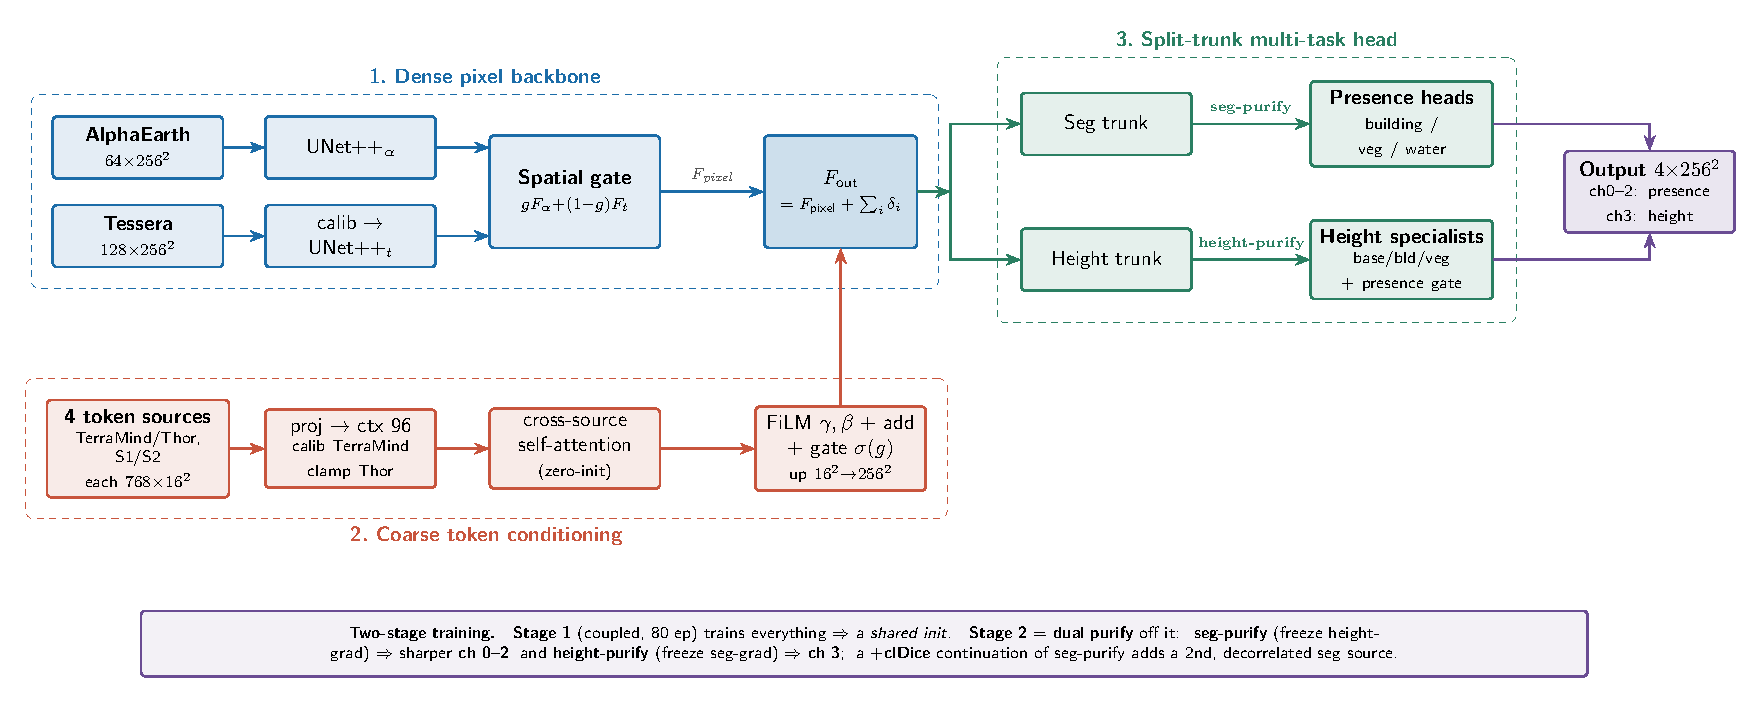
\includegraphics[width=\textwidth]{architecture.pdf}

  \vspace{0.4em}
  {\footnotesize
   \textcolor{cAlpha}{$\blacksquare$ dense pixel}\quad
   \textcolor{cToken}{$\blacksquare$ coarse token}\quad
   \textcolor{cHead}{$\blacksquare$ split head}\quad
   \textcolor{cOut}{$\blacksquare$ output / two-stage}}
\end{frame}

% =====================================================================
\section{Design 1 --- Dense pixel backbone}
% =====================================================================

\begin{frame}{Dual U-Net++ + learned gate \hfill\small\textcolor{cAlpha}{dense path}}
  \begin{center}
  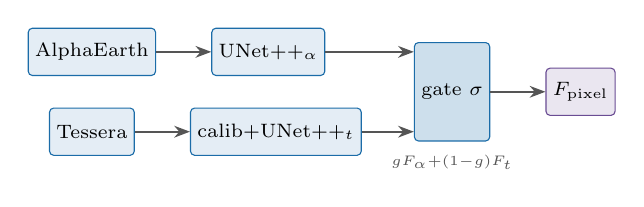
\begin{tikzpicture}[node distance=4mm and 7mm]
    \node[spix] (ae) {AlphaEarth};
    \node[spix,below=of ae] (te) {Tessera};
    \node[spix,right=of ae] (au) {UNet++$_\alpha$};
    \node[spix,right=of te] (tu) {calib+UNet++$_t$};
    \node[sbox,fill=cAlpha!22,draw=cAlpha,minimum height=1.25cm,
          right=18mm of $(au)!0.5!(tu)$] (g) {gate $\sigma$};
    \node[sop,right=7mm of g] (f) {$F_{\text{pixel}}$};
    \draw[sar] (ae)--(au); \draw[sar] (te)--(tu);
    \draw[sar] (au.east) -- (au.east -| g.west);
    \draw[sar] (tu.east) -- (tu.east -| g.west);
    \draw[sar] (g)--(f);
    \node[font=\tiny,cGray,below=0.5mm of g] {$gF_\alpha{+}(1{-}g)F_t$};
  \end{tikzpicture}
  \end{center}
  \begin{itemize}
    \item \fit both are dense $256^2$ $\to$ a U-Net++ yields sharp, IoU-friendly masks.
    \item \fit they differ in reliability $\to$ the gate trusts each per pixel;
      bias init $+4$ $\Rightarrow$ starts AlphaEarth-dominant.
  \end{itemize}
  {\footnotesize ViT / SegFormer / HRNet / UPerNet backbones were all tried and lost.}
\end{frame}

\begin{frame}{Backbone internals}
  \begin{columns}[T]
    \begin{column}{0.54\textwidth}
      \textbf{U-Net++} (\code{base\_ch=48}, LightUNet base)
      \begin{itemize}\small
        \item 4 levels: $48\to96\to192\to384$.
        \item 3$\times$ MaxPool down ($256\to32$), bilinear up + \emph{nested} dense skips.
        \item DoubleConv blocks, BatchNorm.
        \item \code{forward\_features} $\to$ 48-ch map at full res.
      \end{itemize}
    \end{column}
    \begin{column}{0.46\textwidth}
      \textbf{Tessera entry \& gate}
      \begin{itemize}\small
        \item \code{ChannelCalibration}: per-channel affine $x\!\cdot\!s+b$
          (re-normalise the GFM's arbitrary scales).
        \item Gate = \emph{rich} conv$\to$GN$\to$GELU$\to$conv, zero-init weights,
          bias $+4$ (tied: $g$ and $1{-}g$).
      \end{itemize}
    \end{column}
  \end{columns}
\end{frame}

% =====================================================================
\section{Design 2 --- Coarse token conditioning}
% =====================================================================

\begin{frame}{Cross-source token fusion \hfill\small\textcolor{cToken}{coarse path}}
  \begin{center}
  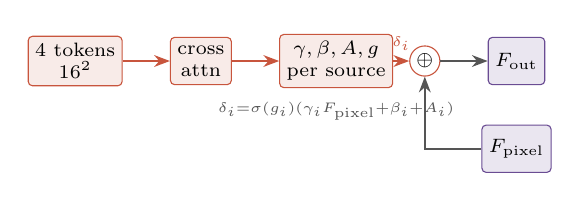
\begin{tikzpicture}[node distance=6mm]
    \node[stok] (t) {4 tokens\\$16^2$};
    \node[stok,right=of t] (a) {cross\\attn};
    \node[stok,right=of a] (m) {$\gamma,\beta,A,g$\\per source};
    \node[sop,draw=cOut,right=12mm of m] (fo) {$F_{\text{out}}$};
    \node[sop,below=5mm of fo] (fp) {$F_{\text{pixel}}$};
    \node[circle,draw=cToken,inner sep=1pt,font=\scriptsize,left=6mm of fo] (s) {$\oplus$};
    \draw[sar,cToken] (t)--(a); \draw[sar,cToken] (a)--(m);
    \draw[sar,cToken] (m)--(s) node[midway,above,font=\tiny,cToken]{$\delta_i$};
    \draw[sar] (fp)-|(s); \draw[sar] (s)--(fo);
    \node[font=\tiny,cGray,below=0.5mm of m,text width=3.2cm,align=center]
         {$\delta_i{=}\sigma(g_i)(\gamma_iF_{\text{pixel}}{+}\beta_i{+}A_i)$};
  \end{tikzpicture}
  \end{center}
  \begin{itemize}
    \item Each source projects to a shared context, cross-attends, then adds a
      zero-init residual (FiLM + additive + gate).
    \item \fit coarse tokens can't make pixels $\to$ they \emph{modulate} the
      dense feature, never replace it.
    \item \fit SAR vs.\ optical see different physics $\to$ attention lets them
      inform each other.
  \end{itemize}
\end{frame}

\begin{frame}{Token fusion internals}
  \begin{columns}[T]
    \begin{column}{0.5\textwidth}
      \textbf{Attend} ($16\times16$)
      \begin{itemize}\small
        \item $1{\times}1$ proj: $768\to$ ctx $96$ per source.
        \item 4-head self-attention over the $4\!\times\!256$ tokens.
        \item learned modality embedding + 2D positional MLP.
        \item \alert{zero-init} output proj $\Rightarrow$ identity at start.
      \end{itemize}
    \end{column}
    \begin{column}{0.5\textwidth}
      \textbf{Inject} ($256\times256$)
      \begin{itemize}\small
        \item bilinear up $16^2\to256^2$, then FiLM+add+gate.
        \item all fusion convs \alert{zero-init}.
        \item run in fp32 for stability.
        \item clamps: token/ctx $\pm50$, FiLM/add $\pm4$.
      \end{itemize}
    \end{column}
  \end{columns}
\end{frame}

\begin{frame}{Respecting each embedding's nature}
  \begin{itemize}
    \item \textbf{Selective calibration.} Calibrate TerraMind (\code{indices=[0,1]});
      leave Thor \emph{uncalibrated + clamped}.\\
      \fit Thor spans $\pm17$k --- calibrating it collapses water IoU.
    \item \textbf{Zero-init injection.} At init $F_{\text{out}}\!\equiv\!F_{\text{pixel}}$.\\
      \fit boots as a pixel-only net, then \emph{earns} token influence; a weak
      source degrades gracefully.
  \end{itemize}
  \vfill
  {\footnotesize Attribution: dropping any of the 4 sources, or any of the 3 pathways, hurt the score.}
\end{frame}

% =====================================================================
\section{Design 3 --- Split-trunk head}
% =====================================================================

\begin{frame}{Split-trunk multi-task head \hfill\small\textcolor{cHead}{head}}
  \begin{center}
  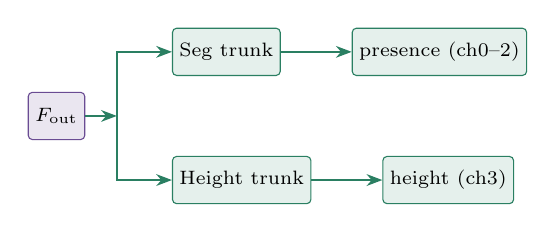
\begin{tikzpicture}[node distance=4mm and 9mm]
    \node[sop] (f) {$F_{\text{out}}$};
    \node[shd,above right=2mm and 11mm of f] (s) {Seg trunk};
    \node[shd,below right=2mm and 11mm of f] (h) {Height trunk};
    \node[shd,right=of s] (p) {presence (ch0--2)};
    \node[shd,right=of h] (hh) {height (ch3)};
    \coordinate (sp) at ($(f.east)+(4mm,0)$);
    \draw[sar,cHead] (f)--(sp);
    \draw[sar,cHead] (sp)|-(s); \draw[sar,cHead] (sp)|-(h);
    \draw[sar,cHead] (s)--(p);  \draw[sar,cHead] (h)--(hh);
  \end{tikzpicture}
  \end{center}
  \begin{itemize}
    \item Two trunks off $F_{\text{out}}$, sharing \emph{no} head weights.
    \item \fit IoU wants crisp masks, RMSE wants smooth regression --- a shared
      trunk makes their gradients fight; splitting lets each shape its features.
    \item Forward is always the full split; what \emph{changes} is how much each
      trunk's gradient reaches the shared backbone --- a per-stage knob (coupled in
      stage-1, one side cut to 0 in the stage-2 purify).
    \item Presence head \emph{is} the metric (BCE on coverage @ 0.5), not a
      reparam of fractions.
  \end{itemize}
\end{frame}

\begin{frame}{Head internals \& the gradient cut}
  \begin{columns}[T]
    \begin{column}{0.5\textwidth}
      \textbf{Trunks \& heads}
      \begin{itemize}\small
        \item trunk = ConvGNAct + residual + GELU.
        \item presence \code{split\_all}: independent head per class
          (\code{branch\_ch 48}, tower depth 2).
        \item height: 3 independent branches (\code{hidden 96}, depth 2).
      \end{itemize}
    \end{column}
    \begin{column}{0.5\textwidth}
      \textbf{Soft gradient decouple}
      \begin{itemize}\small
        \item forward identity:\\ $s\,t+(1{-}s)\,t.\text{detach}()$ --- output
          unchanged; only the backward gradient is scaled.
        \item $s\,{=}\,1$ coupled (stage-1); $s\,{=}\,0$ hard cut (stage-2 purify).
        \item so the ``grad-cut'' is a \emph{stage-2} action, not always on --- it
          is the knob the two-stage recipe flips.
      \end{itemize}
    \end{column}
  \end{columns}
\end{frame}

\begin{frame}{Presence-gated height specialists}
  \begin{center}
  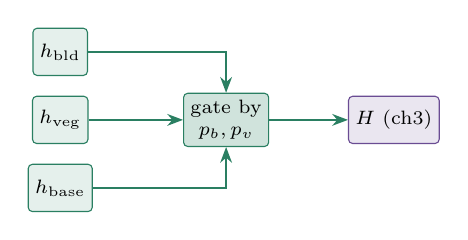
\begin{tikzpicture}[node distance=2.5mm and 10mm]
    \node[shd] (hb) {$h_{\text{bld}}$};
    \node[shd,below=of hb] (hv) {$h_{\text{veg}}$};
    \node[shd,below=of hv] (h0) {$h_{\text{base}}$};
    \node[sbox,fill=cHead!22,draw=cHead,right=12mm of hv] (g)
         {gate by\\$p_b,p_v$};
    \node[sop,right=of g] (H) {$H$ (ch3)};
    \draw[sar,cHead] (hb.east)-|(g.north);
    \draw[sar,cHead] (hv)--(g);
    \draw[sar,cHead] (h0.east)-|(g.south);
    \draw[sar,cHead] (g)--(H);
  \end{tikzpicture}
  \end{center}
  \[ H = p_{\text{fg}}\,(w_b h_{\text{bld}}+w_v h_{\text{veg}})+(1-p_{\text{fg}})h_{\text{base}},
     \quad p_{\text{fg}}{=}1{-}(1{-}p_b)(1{-}p_v) \]
  \begin{itemize}
    \item \fit the metric masks RMSE \emph{per class} --- each specialist is
      L1-trained, and trusted, only on its own class's pixels.
    \item Gate uses \emph{alpha} presence logits; each $h$ comes from the
      soft-bin head (next slide).
  \end{itemize}
\end{frame}

\begin{frame}{Soft-bin height head \hfill\small\textcolor{cHead}{head}}
  Each specialist emits \textbf{64 bin logits}, not a scalar; the height is the
  \textbf{soft-argmax} (expectation over bin centers):
  \[ \hat h = \sum_k \text{softmax}(\ell)_k\,c_k \]
  \begin{columns}[T]
    \begin{column}{0.4\textwidth}
      \centering
      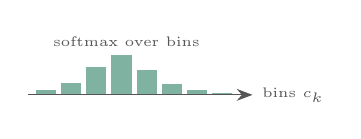
\begin{tikzpicture}[x=0.32cm,y=0.5cm,font=\tiny]
        \foreach \i/\h in {0/0.12,1/0.3,2/0.72,3/1.0,4/0.62,5/0.27,6/0.12,7/0.05}
          {\fill[cHead!60] (\i,0) rectangle (\i+0.8,\h);}
        \draw[->,cGray] (-0.3,0)--(8.6,0) node[right,font=\tiny]{bins $c_k$};
        \node[font=\tiny,cGray] at (3.6,1.35) {softmax over bins};
      \end{tikzpicture}
    \end{column}
    \begin{column}{0.6\textwidth}
      \begin{itemize}\small
        \item \textbf{One shared grid:} log-spaced $[0,80]$\,m, 64 bins ---
          base/bld/veg share the centers (separate conv projections).
        \item bin-CE makes the distribution \emph{commit} to a bin rather than
          collapse to a safe mean (vs.\ L1-only).
        \item Non-negative by construction ($c_k\ge0$).
      \end{itemize}
    \end{column}
  \end{columns}
  \vspace{0.3em}
  {\footnotesize \textcolor{cToken}{Refuted:} per-class grids
   (bld log$[0,160]$, veg \emph{linear}$[0,40]$) --- veg soft-argmax blew up
   (RMSE$_{vH}$ 7.0 vs 2.9), no building gain. Shared grid stays best.}
\end{frame}

% =====================================================================
\section{Design 4 --- Two-stage training}
% =====================================================================

\begin{frame}{Two-stage: train, then purify (1 height + 2 seg)}
  \vspace{-0.3em}
  \begin{center}
  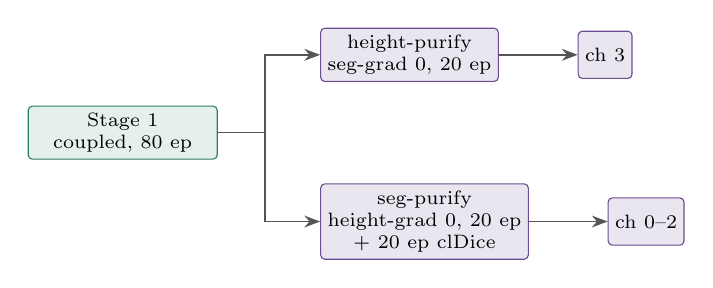
\begin{tikzpicture}[font=\scriptsize,node distance=4mm and 10mm]
    \node[shd,minimum width=2.4cm] (s1) {Stage 1\\coupled, 80 ep};
    \node[sop,above right=3mm and 13mm of s1] (hp) {height-purify\\\scriptsize seg-grad 0, 20 ep};
    \node[sop,below right=3mm and 13mm of s1] (sp) {seg-purify\\\scriptsize height-grad 0, 20 ep\\$+$ 20 ep clDice};
    \node[sbox,fill=cOut!14,draw=cOut,right=10mm of hp] (h3) {ch 3};
    \node[sbox,fill=cOut!14,draw=cOut,right=10mm of sp] (seg) {ch 0--2};
    \coordinate (br) at ($(s1.east)+(6mm,0)$);
    \draw[semithick,cGray] (s1.east) -- (br);   % stub from the box, then branch
    \draw[sar] (br) |- (hp.west);
    \draw[sar] (br) |- (sp.west);
    \draw[sar] (hp.east) -- (h3.west);
    \draw[sar] (sp.east) -- (seg.west);
  \end{tikzpicture}
  \end{center}
  \vspace{-0.9em}
  \begin{columns}[T]
    \begin{column}{0.4\textwidth}
      \textbf{\textcolor{cHead}{Stage 1}} --- coupled, 80 ep\\
      \footnotesize AdamW lr $2{\times}10^{-4}$; train everything jointly
      $\Rightarrow$ a \emph{shared init}.\\[3pt]
      Seg (crisp, IoU) and height (smooth, RMSE) fight over the shared backbone, so
      each purify freezes one task's gradient and lets the other own it (a \emph{mirror}).
    \end{column}
    \begin{column}{0.6\textwidth}
      \textbf{\textcolor{cHead}{Stage 2}} --- purify off stage 1, 20 ep, lr $1.5{\times}10^{-4}$\\
      \footnotesize
      \begin{itemize}\scriptsize
        \item \code{height-purify} (\code{presence-trunk-grad-scale 0}) $\to$ \textbf{ch 3}
        \item \code{seg-purify} (\code{height-trunk-grad-scale 0}), then $+$20 ep clDice
          on top $\to$ \textbf{ch 0--2}
      \end{itemize}
    \end{column}
  \end{columns}
  \vspace{0.2em}
  {\footnotesize \fit $\sim$50 ep already reproduces the 80-ep result within noise
   (Stage 1 keeps its \emph{best-val} checkpoint).}
\end{frame}

\begin{frame}{Stage-2 purify $=$ a one-sided grad-cut \hfill\small\textcolor{cHead}{two-stage}}
  \begin{columns}[T]
    \begin{column}{0.5\textwidth}
      \centering
      \textbf{\textcolor{cHead}{height-purify}}\\
      {\footnotesize\code{presence-trunk-grad-scale 0}}\\[4pt]
      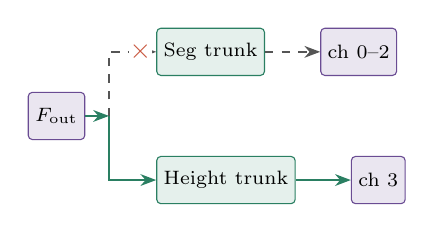
\begin{tikzpicture}[node distance=2.5mm and 8mm,font=\scriptsize]
        \node[sop] (f) {$F_{\text{out}}$};
        \node[shd,above right=2mm and 9mm of f] (s) {Seg trunk};
        \node[shd,below right=2mm and 9mm of f] (h) {Height trunk};
        \node[sbox,fill=cOut!14,draw=cOut,right=7mm of s] (p) {ch 0--2};
        \node[sbox,fill=cOut!14,draw=cOut,right=7mm of h] (hh) {ch 3};
        \coordinate (sp) at ($(f.east)+(3mm,0)$);
        \draw[sar,cHead] (f)--(sp);
        \draw[sar,cGray,dashed] (sp)|-(s);
        \draw[sar,cHead] (sp)|-(h);
        \draw[sar,cGray,dashed] (s)--(p);
        \draw[sar,cHead] (h)--(hh);
        \node[cToken,font=\normalsize\bfseries,fill=white,inner sep=0.4pt]
          at ([xshift=-2mm]s.west) {$\times$};
      \end{tikzpicture}\\[3pt]
      {\footnotesize seg gradient cut $\Rightarrow$ height re-tunes the backbone.}
    \end{column}
    \begin{column}{0.5\textwidth}
      \centering
      \textbf{\textcolor{cHead}{seg-purify}} (mirror)\\
      {\footnotesize\code{height-trunk-grad-scale 0}}\\[4pt]
      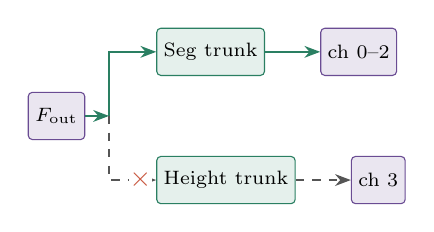
\begin{tikzpicture}[node distance=2.5mm and 8mm,font=\scriptsize]
        \node[sop] (f) {$F_{\text{out}}$};
        \node[shd,above right=2mm and 9mm of f] (s) {Seg trunk};
        \node[shd,below right=2mm and 9mm of f] (h) {Height trunk};
        \node[sbox,fill=cOut!14,draw=cOut,right=7mm of s] (p) {ch 0--2};
        \node[sbox,fill=cOut!14,draw=cOut,right=7mm of h] (hh) {ch 3};
        \coordinate (sp) at ($(f.east)+(3mm,0)$);
        \draw[sar,cHead] (f)--(sp);
        \draw[sar,cHead] (sp)|-(s);
        \draw[sar,cGray,dashed] (sp)|-(h);
        \draw[sar,cHead] (s)--(p);
        \draw[sar,cGray,dashed] (h)--(hh);
        \node[cToken,font=\normalsize\bfseries,fill=white,inner sep=0.4pt]
          at ([xshift=-2mm]h.west) {$\times$};
      \end{tikzpicture}\\[3pt]
      {\footnotesize height gradient cut $\Rightarrow$ seg owns the backbone.}
    \end{column}
  \end{columns}
  \vspace{0.5em}
  {\footnotesize \fit forward is unchanged (identity) --- the \textcolor{cToken}{$\times$}
   blocks only that trunk's \emph{gradient} into the shared backbone, so each purify hands
   the backbone to one task. (\code{grad-scale} $1{=}$coupled, $0{=}$cut.)}
\end{frame}

% =====================================================================
\section{Loss}
% =====================================================================

\begin{frame}{Loss --- every term tracks the metric}
  \code{ImprovedCompositeLoss} (presence-centered):
  \begin{center}\small
  \begin{tabular}{lll}
    \toprule
    Term & Target & Metric\\
    \midrule
    Presence BCE (ring-weighted) & presence logits & IoU\\
    Presence Tversky ($\alpha$ per class) & presence prob & IoU prec/recall\\
    Height L1 + bin-CE & soft-bin specialists & RMSE\\
    Building-boundary BCE+Dice & aux edge head & IoU edges\\
    Water empty top-$k$ & water logits & water IoU (FP)\\
    \bottomrule
  \end{tabular}
  \end{center}
  \footnotesize Weights: bld height boost $\times5$, veg $\times1.5$; bin-CE $0.5$;
  bg weight $0.05$; ring $\alpha{=}2$ (k5); water top-$k$ 512 @ $0.03$; boundary $0.25$.
\end{frame}

\begin{frame}{Height loss: L1 + bin-CE}
  \begin{columns}[T]
    \begin{column}{0.36\textwidth}
      \centering
      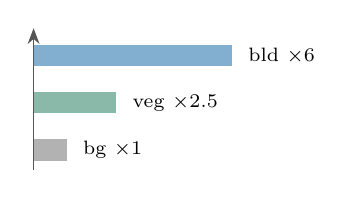
\begin{tikzpicture}[x=0.42cm,y=0.6cm,font=\scriptsize]
        \fill[cAlpha!55] (0,2) rectangle (6,2.45);
          \node[anchor=west] at (6.2,2.22) {bld $\times6$};
        \fill[cHead!55] (0,1) rectangle (2.5,1.45);
          \node[anchor=west] at (2.7,1.22) {veg $\times2.5$};
        \fill[cGray!45] (0,0) rectangle (1,0.45);
          \node[anchor=west] at (1.2,0.22) {bg $\times1$};
        \draw[->,cGray] (0,-0.2)--(0,2.8);
      \end{tikzpicture}\\[3pt]
      {\scriptsize L1 weight $1+5m_{\text{bld}}+1.5m_{\text{veg}}$}
    \end{column}
    \begin{column}{0.64\textwidth}
      Heights normalised $/30$\,m. Two terms:
      \begin{itemize}\small
        \item \textbf{L1} $|\hat h-h|$ on the soft-argmax height: blended output
          (weights, left) + per-class aux on own-class pixels.
        \item \textbf{bin-CE} ($0.5$): Gaussian soft-target over bins ($\sigma{=}1.5$)
          vs.\ predicted bin distribution $\to$ \emph{commit} to the right bin,
          not collapse to a safe mean. \textcolor{cHead}{(the key soft-bin term)}
        \item \textbf{Base} specialist: bin-CE over \emph{all} valid pixels +
          blended L1 $\to$ bg/water height ($\approx0$) is still constrained,
          just not metric-scored.
      \end{itemize}
    \end{column}
  \end{columns}
  \vspace{0.1em}
  {\footnotesize Masks use \code{gt\_class>thr} --- the same per-class mask the RMSE metric scores on.}
\end{frame}

\begin{frame}{Ring-weighted presence BCE}
  \begin{columns}[T]
    \begin{column}{0.4\textwidth}
      \centering
      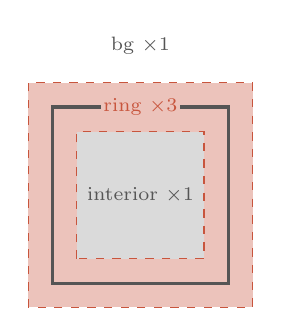
\begin{tikzpicture}[scale=0.95]
        \fill[cToken!35] (-1.5,-1.5) rectangle (1.5,1.5);   % ring band
        \fill[cGray!22]  (-0.85,-0.85) rectangle (0.85,0.85); % interior
        \draw[dashed,cToken] (-1.5,-1.5) rectangle (1.5,1.5);  % dilate
        \draw[dashed,cToken] (-0.85,-0.85) rectangle (0.85,0.85); % erode
        \draw[very thick,cGray] (-1.18,-1.18) rectangle (1.18,1.18); % mask edge
        \node[font=\scriptsize,cGray,align=center] at (0,0) {interior $\times1$};
        \node[font=\scriptsize,cToken,fill=cToken!35,inner sep=1pt] at (0,1.18) {ring $\times3$};
        \node[font=\scriptsize,cGray] at (0,2.0) {bg $\times1$};
      \end{tikzpicture}\\[2pt]
      {\scriptsize dashed = dilate / erode (k5); solid = mask edge}
    \end{column}
    \begin{column}{0.6\textwidth}
      \begin{itemize}
        \item \textbf{ring} $=$ dilate$(m)-$erode$(m)$: a $\pm2$px band on the
          building edge.
        \item weight $w = 1 + 2\cdot\text{ring}$ $\Rightarrow$ ring pixels count
          $3\times$, all else $1\times$ (only the building channel).
        \item \fit 88\% of lost building IoU sits in this band; equal weighting
          lets the easy interior/bg dominate.
        \item Reweights the \emph{main} presence logit (what IoU reads), not a
          separate boundary head.
      \end{itemize}
    \end{column}
  \end{columns}
\end{frame}

\begin{frame}{clDice --- a topology loss for merged buildings}
  \begin{columns}[T]
    \begin{column}{0.52\textwidth}
      \textbf{The failure it targets}
      \begin{itemize}\small
        \item Buildings are 1--2\,px wide; the model \emph{merges} adjacent ones
          (predicts 67 components/tile vs.\ GT's 104).
        \item \textbf{51\% of building FP} is inter-building ``bridges'';
          oracle un-merge $\to$ IoU $0.504\!\to\!0.587$.
      \end{itemize}
    \end{column}
    \begin{column}{0.48\textwidth}
      \textbf{clDice} (\code{cl-dice-weight})
      \begin{itemize}\small
        \item \code{soft\_skeleton}: a differentiable skeleton via iterated
          min/max-pool (no parameters), then centerline Dice on the building
          presence map.
        \item rewards \emph{connectivity}, penalises merges --- orthogonal to the
          area (Tversky) losses.
        \item applied only as a late 20-ep purify (not in stage-1).
      \end{itemize}
    \end{column}
  \end{columns}
  \vspace{0.3em}
  {\footnotesize \textcolor{cToken}{Not in stage-1:} baking clDice into stage-1 pulled
   the backbone toward topology and \emph{degraded height} (RMSE$_{bH}$ +0.006); the
   late-purify placement keeps height untouched.}
\end{frame}

% =====================================================================
\section{Inference \& Results}
% =====================================================================

\begin{frame}{Inference}
  \begin{itemize}
    \item \textbf{5-fold, leave-region-out CV} --- so local val predicts the
      public board (LB $\approx$ worst fold).
    \item \textbf{Mean ensemble} across folds; optional 0.3 water-expert blend.
    \item \textbf{Per-class threshold sweep} on OOF, then binarize\\
      (bld $0.775$ / veg $0.675$ / water $0.725$).
    \item \fit IoU is judged at a hard cut, different per class $\to$ tune each
      on held-out data.
  \end{itemize}
  \vfill
  {\footnotesize Ruled out (tried, no gain): TTA, D4 aug, bigger ensembles, region-conditioning.}
\end{frame}

\begin{frame}{Final model: \code{xf095\_2stage\_softbin\_covgt10}}
  Two-stage dual-trunk + shared soft-bin.
  5-fold (seed 0), purify checkpoints:
  \begin{center}\small
  \begin{tabular}{lccccc}
    \toprule
    fold & Score & iou\_bld & iou\_wat & RMSE$_{bH}$ & RMSE$_{vH}$\\
    \midrule
    f0 & 0.509 & 0.511 & 0.455 & 1.60 & 2.92\\
    f1 & 0.541 & 0.512 & 0.466 & 1.40 & 2.70\\
    f2 & 0.521 & 0.497 & 0.448 & 1.48 & 2.78\\
    f3 & 0.530 & 0.500 & 0.465 & 1.43 & 2.74\\
    f4 & 0.525 & 0.522 & 0.468 & 1.48 & 2.93\\
    \midrule
    \textbf{mean} & \textbf{0.525} & & & &\\
    \bottomrule
  \end{tabular}
  \end{center}
  \footnotesize Worst fold f0 $0.509$ $\approx$ public LB. Building IoU still
  boundary-limited (88\% of lost IoU in a $\pm2$px band); that is the open lever.
\end{frame}

% =====================================================================
\section{Final Submission}
% =====================================================================

\begin{frame}{From one model to the final ensemble}
  Everything above is \emph{one} model. The submitted system ensembles
  \textbf{5 architectures $\times$ 5 folds}, each run through \textbf{3 training
  stages}:
  \begin{center}\small
  \begin{tabular}{lll}
    \toprule
    Member & \code{pixel\_backbone} & seeds\\
    \midrule
    U-Net++ (nested decoder) & \code{unetpp} & 0,\,1,\,2\\
    UNet\,3+ (full-scale skip) & \code{unet3plus} & 0\\
    TransUNet (attn bottleneck) & \code{unetpp\_trans} & 0\\
    \bottomrule
  \end{tabular}
  \end{center}
  \begin{itemize}\small
    \item \fit identical inputs $\Rightarrow$ \emph{architecture} diversity
      decorrelates errors better than more seeds of one net.
    \item 5-fold leave-region-out; the ensemble is a plain mean of member-fold
      probability maps, then thresholded.
  \end{itemize}
  {\footnotesize U-Net++ was the only backbone that beat plain LightUNet on the
   official IoU metric; heavier/attention encoders all lost.}
\end{frame}

\begin{frame}{Seg from two decorrelated sources (50-member)}
  Final channels:
  \begin{itemize}\small
    \item \textbf{seg ch 0--2} $=$ mean of \textbf{50} member-folds
      $=$ 25 clDice $\cup$ 25 seg-purify (the two share a stage-1 but diverge in
      the seg fine-tune $\Rightarrow$ decorrelated).
    \item \textbf{height ch 3} $=$ mean of \textbf{25} height-purify member-folds
      \emph{only} (adding stage-1 height \emph{hurt} --- it is strictly worse).
  \end{itemize}
  \vspace{0.3em}
  \fit pure variance reduction --- no parameter is tuned on the public board, so
  it transfers to the private split. On public it lifted all three IoUs
  (bld $+0.0013$, veg $+0.0011$, water $+0.0015$).
\end{frame}

\begin{frame}{Height calibration: explaining the local$\to$public gap}
  Local (OOF, tile-RMSE) vs.\ public, \emph{no shift}:
  \begin{center}\small
  \begin{tabular}{lccc}
    \toprule
    & OOF tile & OOF pixel & public\\
    \midrule
    RMSE$_{bH}$ & 1.48 & 2.32 & 1.81\\
    RMSE$_{vH}$ & 2.74 & 2.97 & 3.08\\
    \bottomrule
  \end{tabular}
  \end{center}
  \begin{itemize}\small
    \item \textbf{Convention is tile-based}: the tile gap is a \emph{consistent}
      $+0.33$\,m on \emph{both} heights (region shift); the pixel gap is
      inconsistent (building would improve --- impossible).
    \item \textbf{Mechanism}: soft-argmax \emph{range compression} (tall
      under-predicted) $\times$ a taller test region $\Rightarrow$ systematic
      under-prediction.
  \end{itemize}
\end{frame}

\begin{frame}{Height correction: per-class calibration (applied in final)}
  \begin{columns}[T]
    \begin{column}{0.5\textwidth}
      \textbf{Building: de-compression} \textcolor{cHead}{(used)}
      \begin{itemize}\small
        \item $h\!\to\!1.05h+0.116$ (slope $>1$, un-squeeze the compressed tall tail).
        \item motivated by the strong compression curve ($-4.5$\,m @ 15\,m).
        \item region-invariant $\Rightarrow$ private-safe. RMSE$_{bH}$ $1.807\!\to\!1.782$.
      \end{itemize}
    \end{column}
    \begin{column}{0.5\textwidth}
      \textbf{Vegetation: additive shift} \textcolor{cHead}{(used)}
      \begin{itemize}\small
        \item $h\!\to\!h+0.12$ on predicted-veg pixels (pure mean offset).
        \item corrects the small public veg bias. RMSE$_{vH}$ $3.079\!\to\!3.072$.
      \end{itemize}
    \end{column}
  \end{columns}
  \vspace{0.3em}
  {\footnotesize Both corrections are region-invariant (a mean offset, plus a mild
   slope for buildings), not public-fitted; the residual $+0.33$\,m is irreducible
   region-shift scatter.}
\end{frame}

\begin{frame}{Final result \& trajectory}
  \begin{center}\small
  \begin{tabular}{lcccccc}
    \toprule
    Submission & Score & bld & veg & wat & RMSE$_{bH}$ & RMSE$_{vH}$\\
    \midrule
    3-seed U-Net++           & 0.5018 & 0.498 & 0.820 & 0.521 & 1.807 & 3.079\\
    5-member arch ensemble   & 0.5026 & 0.498 & 0.819 & 0.526 & 1.804 & 3.079\\
    +\,seg-purify +\,bld shift & 0.5061 & 0.502 & 0.821 & 0.525 & 1.778 & 3.079\\
    +\,clDice +\,veg shift     & 0.5063 & 0.502 & 0.820 & 0.526 & 1.778 & 3.072\\
    \textbf{+\,50-seg (final)} & \textbf{0.5067} & \textbf{0.503} & \textbf{0.821} & \textbf{0.527} & 1.782 & 3.072\\
    \bottomrule
  \end{tabular}
  \end{center}
  \begin{itemize}\small
    \item \textbf{+0.0049} over the session; the gains are robust (variance
      reduction + a region-invariant mean shift), not public-fitted.
    \item Private $=$ best-public auto-selected $\Rightarrow$ near the end only
      \emph{non-public-tuned} levers were used.
  \end{itemize}
\end{frame}

\begin{frame}{Ablation log --- what moved the needle, what didn't}
  \begin{columns}[T]
    \begin{column}{0.5\textwidth}
      \textcolor{cHead}{\textbf{Kept (each +):}}
      \begin{itemize}\small
        \item cross-architecture ensemble
        \item seg-purify (dedicated seg backbone)
        \item clDice topology loss
        \item per-class height calibration (bld de-comp $1.05h{+}0.116$, veg $+0.12$)
        \item 50-member dual-source seg
        \item delmask (drop human-deleted footprints)
      \end{itemize}
    \end{column}
    \begin{column}{0.5\textwidth}
      \textcolor{cToken}{\textbf{Refuted (tried, no gain):}}
      \begin{itemize}\small
        \item ViT / SegFormer / HRNet / UPerNet / UNet3+\,(solo)
        \item wavelet down-sampling; deep supervision
        \item clDice-from-stage-1
        \item per-code thresholds; morphology; valley-cut
        \item distance-watershed (1--2px $\Rightarrow$ degenerate)
        \item AdaBN; region-conditioning; TTA; D4 aug
      \end{itemize}
    \end{column}
  \end{columns}
  \vspace{0.2em}
  {\footnotesize Building IoU is at the \emph{embedding-resolution} ceiling
   (1--2px buildings); the gap to the top teams is a structural model-quality
   difference (better building-seg / veg-height models on identical embeddings).}
\end{frame}

% =====================================================================
\section{Summary}
% =====================================================================

\begin{frame}{Summary --- each design answers ``what is the input?''}
  \small
  \begin{tabular}{ll}
    \toprule
    \textbf{Design} & \textbf{Driven by\dots}\\
    \midrule
    Dual U-Net++ + gate & dense $256^2$, differing reliability\\
    Cross-source token FiLM & coarse $16^2$ context (modulate, not pixels)\\
    Selective calib + zero-init & wild scales (Thor); optional correction\\
    Split-trunk head & IoU-crisp vs.\ RMSE-smooth conflict\\
    Presence-gated height & per-class RMSE mask\\
    Two-stage purify & conflict reaches the backbone\\
    Per-class threshold sweep & IoU judged at a hard per-class cut\\
    \bottomrule
  \end{tabular}
\end{frame}

\end{document}
